% pcb_homogenization -- module overview with example results
% Compile:  latexmk -pdf main.tex      (or: pdflatex main.tex, twice)
% Figures:  python docs/overview/make_figures.py data/samples/<sample>   (from the repo root)

\documentclass[10pt,a4paper]{article}

\usepackage[T1]{fontenc}
\usepackage[utf8]{inputenc}
\usepackage[scaled=0.95]{helvet}
\renewcommand{\familydefault}{\sfdefault}
\usepackage[scaled=0.9]{inconsolata}
\usepackage[a4paper,margin=18mm,bottom=22mm]{geometry}
\usepackage{graphicx}
\usepackage{xcolor}
\usepackage{booktabs}
\usepackage{tabularx}
\usepackage{array}
\usepackage{siunitx}
\usepackage{caption}
\usepackage{subcaption}
\usepackage{titlesec}
\usepackage{fancyhdr}
\usepackage{enumitem}
\usepackage{float}
\usepackage[hidelinks]{hyperref}

\definecolor{ink}{HTML}{1D232B}
\definecolor{muted}{HTML}{5B6470}
\definecolor{accent}{HTML}{C8702A}
\definecolor{codebg}{HTML}{F3F4F6}

\color{ink}
\setlength{\parindent}{0pt}
\setlength{\parskip}{4pt}
\setlength{\emergencystretch}{3em}
\sisetup{range-phrase=--, range-units=single, mode=match, reset-text-family=false,
         reset-text-series=false, text-family-to-math=true}

\titleformat{\section}{\large\bfseries}{\textcolor{accent}{\thesection}}{0.6em}{}
\titlespacing*{\section}{0pt}{10pt}{4pt}
\titleformat{\subsection}{\normalsize\bfseries}{}{0pt}{}
\titlespacing*{\subsection}{0pt}{8pt}{2pt}

\captionsetup{font={small,color=muted},labelfont=bf,labelsep=endash,justification=raggedright,singlelinecheck=false}

\pagestyle{fancy}
\fancyhf{}
\renewcommand{\headrulewidth}{0pt}
\fancyfoot[L]{\scriptsize\color{muted}pcb\_homogenization v0.1.2 \textperiodcentered{} module overview \textperiodcentered{} MikroVAL internal}
\fancyfoot[R]{\scriptsize\color{muted}\thepage}

% Monospace file/function names; allow a line break after "_", "/" and "." so long names never overflow.
\newcommand{\brkus}{\textunderscore\allowbreak}
\newcommand{\code}[1]{{\small\ttfamily\let\_\brkus #1}}
\newcommand{\mod}[1]{\code{#1}}

\begin{document}

% ---------------------------------------------------------------------------
{\LARGE\bfseries pcb\_homogenization}\\[2pt]
{\small\color{muted} PCB copper-layout homogenization and solder-joint thermal-cycling simulation
\textperiodcentered{} module overview with example results}

\subsection*{What it does}
A 2-layer PCB layout (Gerber) is rasterized into copper/FR4 maps, coarse-grained by a quadtree
with per-leaf Voigt--Reuss homogenization, and mapped onto an ANSYS MAPDL board model. A partner-supplied
CR0805 resistor is placed on the board with SAC305 solder, the assembly is driven through a reflow and
thermal-cycling profile with creep, and the solder creep strain is post-processed per cycle as input for a
fatigue-life law.

\subsection*{Pipeline}
\colorbox{codebg}{\parbox{\dimexpr\linewidth-2\fboxsep}{\footnotesize
\begin{tabular}{@{}l@{\quad}l@{\quad}l@{}}
1 & \code{import\_real\_board.py}  & Gerber $\rightarrow$ sample folder \\
2 & \code{discretize.py}              & copper rasters $\rightarrow$ \code{mesh/F\_Cu\_map.npy}, \code{B\_Cu\_map.npy} \\
3 & \code{quadtree.py}                & Voigt--Reuss leaves $\rightarrow$ \code{mesh/quadtree.json} \\
4 & \code{simulate\_pyansys\_assembly.py} & MAPDL solve $\rightarrow$ \code{results/pyansys\_assembly.rst}, \code{thermal\_profile.yaml/.png} \\
5 & \code{zone\_creep\_strain.py}     & critical-zone creep strain $\rightarrow$ \code{results/zone\_creep\_strain.json} \\
6 & \code{plot\_cycle\_creep\_increment.py} & $\Delta\varepsilon$ per cycle $\rightarrow$ \code{results/cycle\_creep\_increment.json} \\
\end{tabular}
}}

\subsection*{Example used throughout}
Board \code{rv3032\_example} (\qtyproduct{20 x 15}{\milli\metre}, Cu \SI{35}{\micro\metre} / FR4 \SI{1.53}{\milli\metre}),
solved with the shortened example profile \code{configs/thermal\_profile\_example.yaml}
(cool-down from the stress-free \SI{180}{\celsius} to \SI{22}{\celsius} with a \SI{300}{\second} hold, then one
\SIrange{-40}{125}{\celsius} cycle), a \numproduct{20 x 20} board mesh and 8 cores: about \SI{8.5}{\minute}
wall time, 60 substeps, \SI{0.6}{\giga\byte} result file.

\subsection*{Module map}
{\small
\begin{tabularx}{\linewidth}{@{}>{\ttfamily\footnotesize}p{55mm}X@{}}
\toprule
import\_real\_board.py           & Imports real F\_Cu/B\_Cu Gerbers, shifts them to a (0,0) origin, writes \code{metadata.json}. \\
discretize.py                    & Parses RS-274X Gerber copper layers and rasterizes them to binary maps. \\
homogenization.py                & Material loading, Voigt/Reuss bounds. \\
quadtree.py                      & 2:1-balanced (or leaf-budget) quadtree with per-leaf homogenized properties. \\
plot\_board\_model.py            & Top view of the simulated board (projected or homogenized), read from the \code{.rst}. \\
solder\_reliability.py           & Tracked component pads; quick analytical CTE-mismatch / Coffin--Manson estimate. \\
simulate\_pyansys\_benchmark.py  & Board-only MAPDL model: structured hex mesh painted from the rasters. \\
component\_import.py             & Imports the partner \code{.cdb} component, remaps material IDs, MPC bonded contact. \\
simulate\_pyansys\_assembly.py   & Board + CR0805 + SAC305 assembly, thermal profile, creep solve. \\
thermal\_profile.py              & Loads, plots and applies the time/temperature YAML (time table, one load step per segment); cycle boundaries. \\
plot\_creep\_strain\_history.py  & Maximum/mean solder creep strain vs.\ time. \\
zone\_creep\_strain.py           & Critical-zone volume-averaged creep strain (Schwerz / Darveaux method). \\
plot\_cycle\_creep\_increment.py & Per-cycle creep-strain increment $\Delta\varepsilon$ for the fatigue law. \\
plot\_component\_materials.py    & 3-D render of the assembly coloured by material. \\
\bottomrule
\end{tabularx}
}

\newpage
% ---------------------------------------------------------------------------
\section{Board input}
\mod{import\_real\_board.py} converts an externally authored board into the common sample layout
(\code{metadata.json} + \code{gerber/}): it copies the top and bottom copper Gerbers, shifts them so the board
starts at (0,0), and records the stackup. Only the two outer copper layers and the dielectric core are kept.

\section{Discretization}
\mod{discretize.py} parses each RS-274X copper layer (pads, traces, regions) and rasterizes it onto a
uniform grid (\code{-{}-resolution 40} px/mm $\rightarrow$ \numproduct{800 x 600} px here; default 10) and writes \code{F\_Cu\_map.npy},
\code{B\_Cu\_map.npy} and \code{discretization.json}. The top layer carries the signal traces and the
resistor pads (R1, blue markers); the bottom layer is a ground pour with clearances.

\begin{figure}[H]
  \centering
  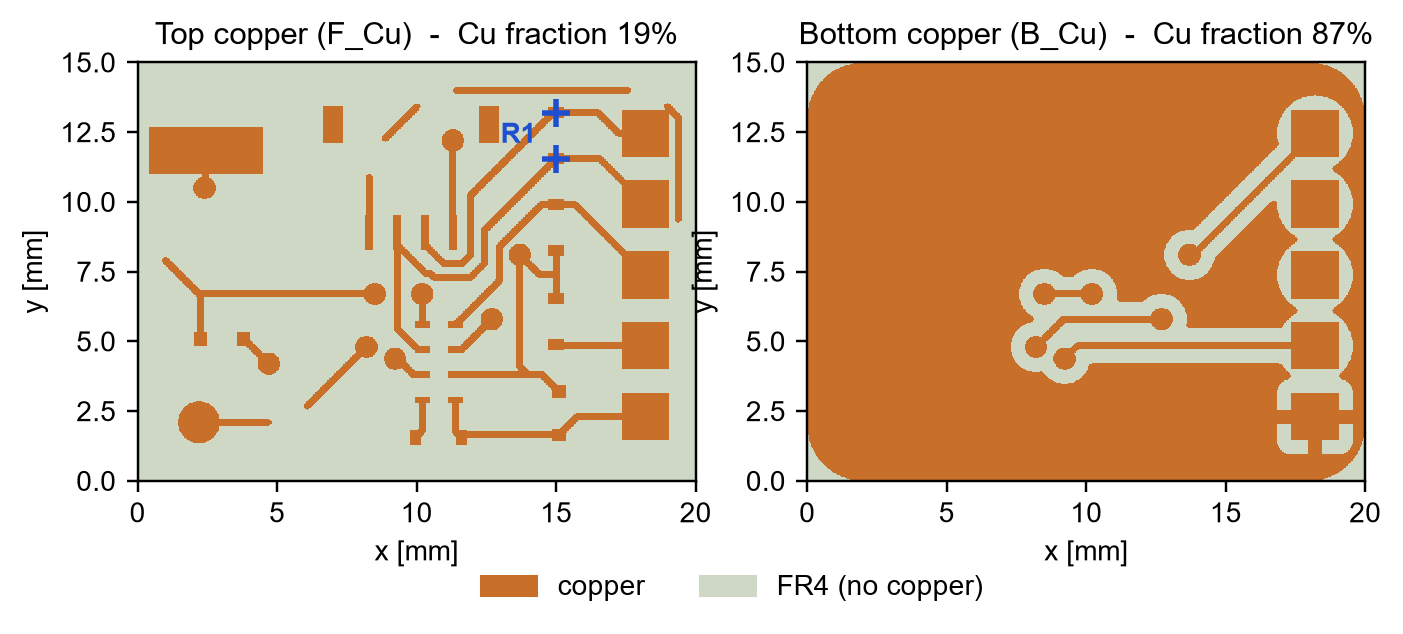
\includegraphics[width=\linewidth]{figures/input_layers.png}
  \caption{Input copper layers of \code{rv3032\_example} after rasterization. Blue crosses: R1 pad centres
  used for component placement (\code{solder\_reliability.py}).}
  \label{fig:layers}
\end{figure}

\section{Homogenization (quadtree)}
\mod{quadtree.py} splits the board wherever a leaf straddles a copper/FR4 boundary (pure leaves are already
exact) and enforces 2:1 balance, or alternatively stops at a leaf budget (\code{-{}-max-leaves}). Each leaf
gets Voigt (in-plane) and Reuss (out-of-plane) stiffness and CTE from its top/bottom copper fractions
(\code{homogenization.voigt\_reuss\_bounds()}). Output: \code{mesh/quadtree.json}.

The MAPDL board model does not use these homogenized properties: it projects the layout directly onto its
elements (Section~\ref{sec:mapping}). \code{mesh/quadtree.json} currently feeds only the quick analytical
CTE-mismatch estimate in \mod{solder\_reliability.py}.

\newpage
% ---------------------------------------------------------------------------
\section{Trace mapping onto the MAPDL board mesh}
\label{sec:mapping}
\mod{simulate\_pyansys\_benchmark.py} builds a structured hex mesh of the board (bottom Cu / FR4 core /
top Cu; nodes and elements created directly via PyMAPDL) and paints each element copper or FR4 by sampling
the raster at the element centre. The mesh density (\code{-{}-nx}, \code{-{}-ny}) therefore decides how much of
the layout survives: at \numproduct{50 x 50} (\qtyproduct{0.4 x 0.3}{\milli\metre} elements) the traces are still
recognizable, at \numproduct{20 x 20} most thin traces vanish and only pads and wide features remain.

\begin{figure}[H]
  \centering
  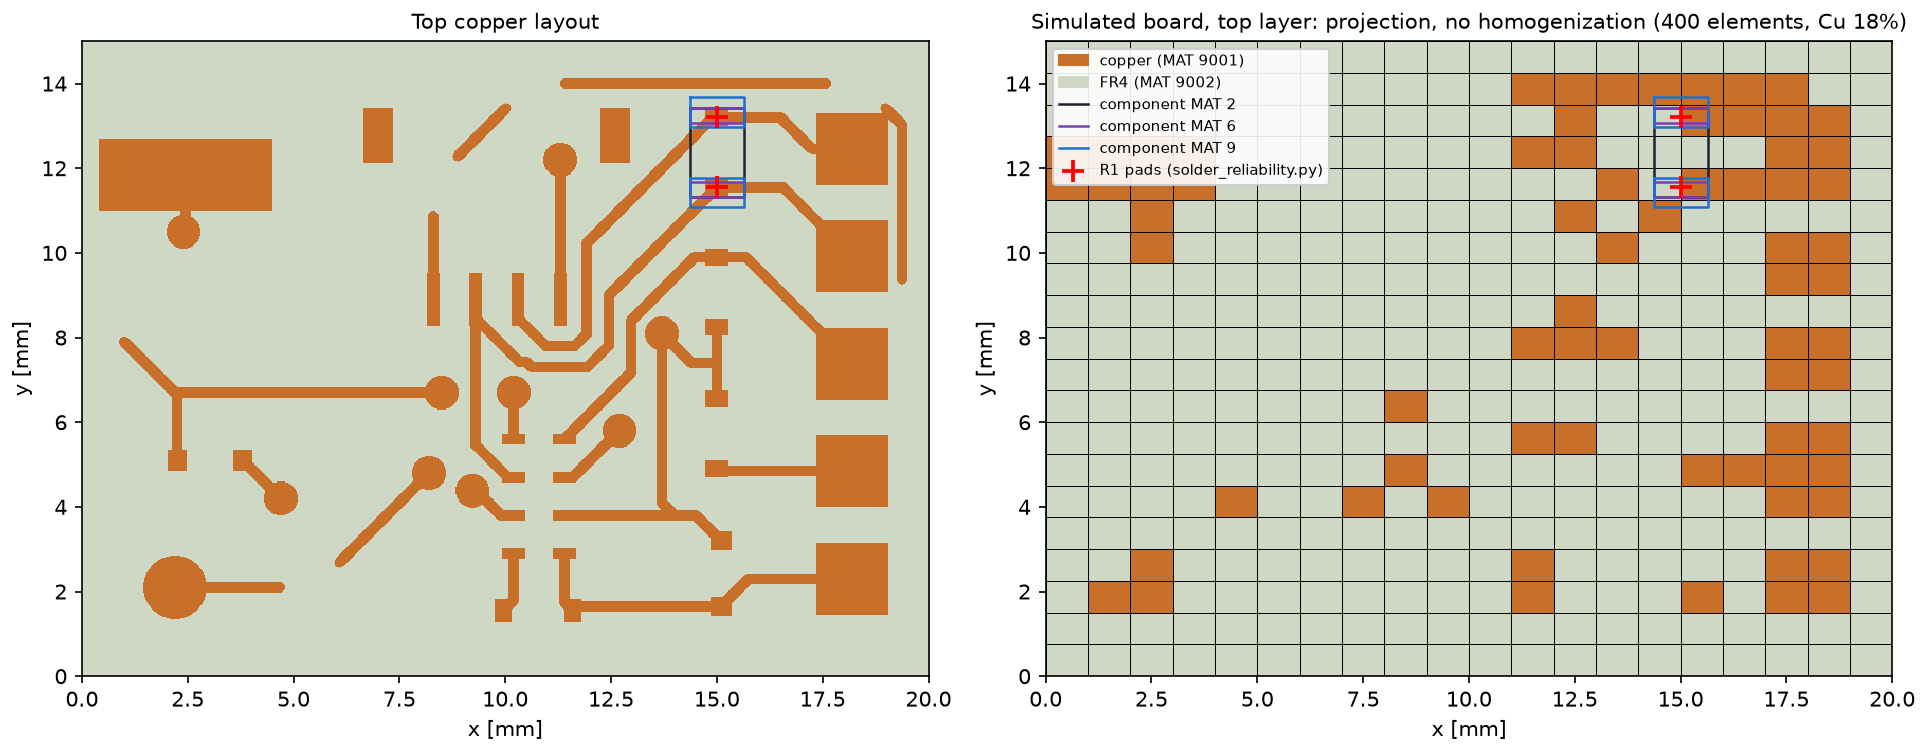
\includegraphics[width=\linewidth]{figures/board_model.png}
  \caption{Top copper layout (left) and the top copper layer of the board as it was simulated (right),
  read back from the result file by \code{plot\_board\_model.py}: \numproduct{20 x 20} elements, each pure
  copper or pure FR4 (no homogenization). Outlines: the simulated CR0805 body (MAT 2), terminations (MAT 6)
  and solder (MAT 9); red crosses: the R1 pad centres used for placement. For a homogenized board the right panel shows the per-element
  in-plane modulus as a colormap instead.}
  \label{fig:mapping}
\end{figure}

\section{Component and solder}
\mod{component\_import.py} reads the partner-supplied CR0805 archive
(\code{DemonstratorB\_CR0805\_Export.cdb}) into the running MAPDL session without remeshing it. Board
materials are moved to MAT 9001/9002 first so they cannot collide with the archive's own material IDs, and
the SAC305 solder law (elastic + creep) is applied from \code{SAC305\_MikroVal.mac}.
\mod{simulate\_pyansys\_assembly.py} places the component at the midpoint of the two R1 pads
(\code{PAD\_1\_XY\_MM}/\code{PAD\_2\_XY\_MM} in \code{solder\_reliability.py}, taken from the Gerber), turns it
onto the pad axis (here \SI{90}{\degree}), drops the solder onto the board's top surface and connects it via MPC
bonded contact, reusing the TARGE170/CONTA174 template from the archive. R1 is an 0603 footprint
(\qtyproduct{0.55 x 0.40}{\milli\metre} pads, \SI{1.65}{\milli\metre} apart) while the archive is a CR0805, so
the component overhangs the pads; Fig.~\ref{fig:mapping} shows its outline on the layout.

\begin{figure}[H]
  \centering
  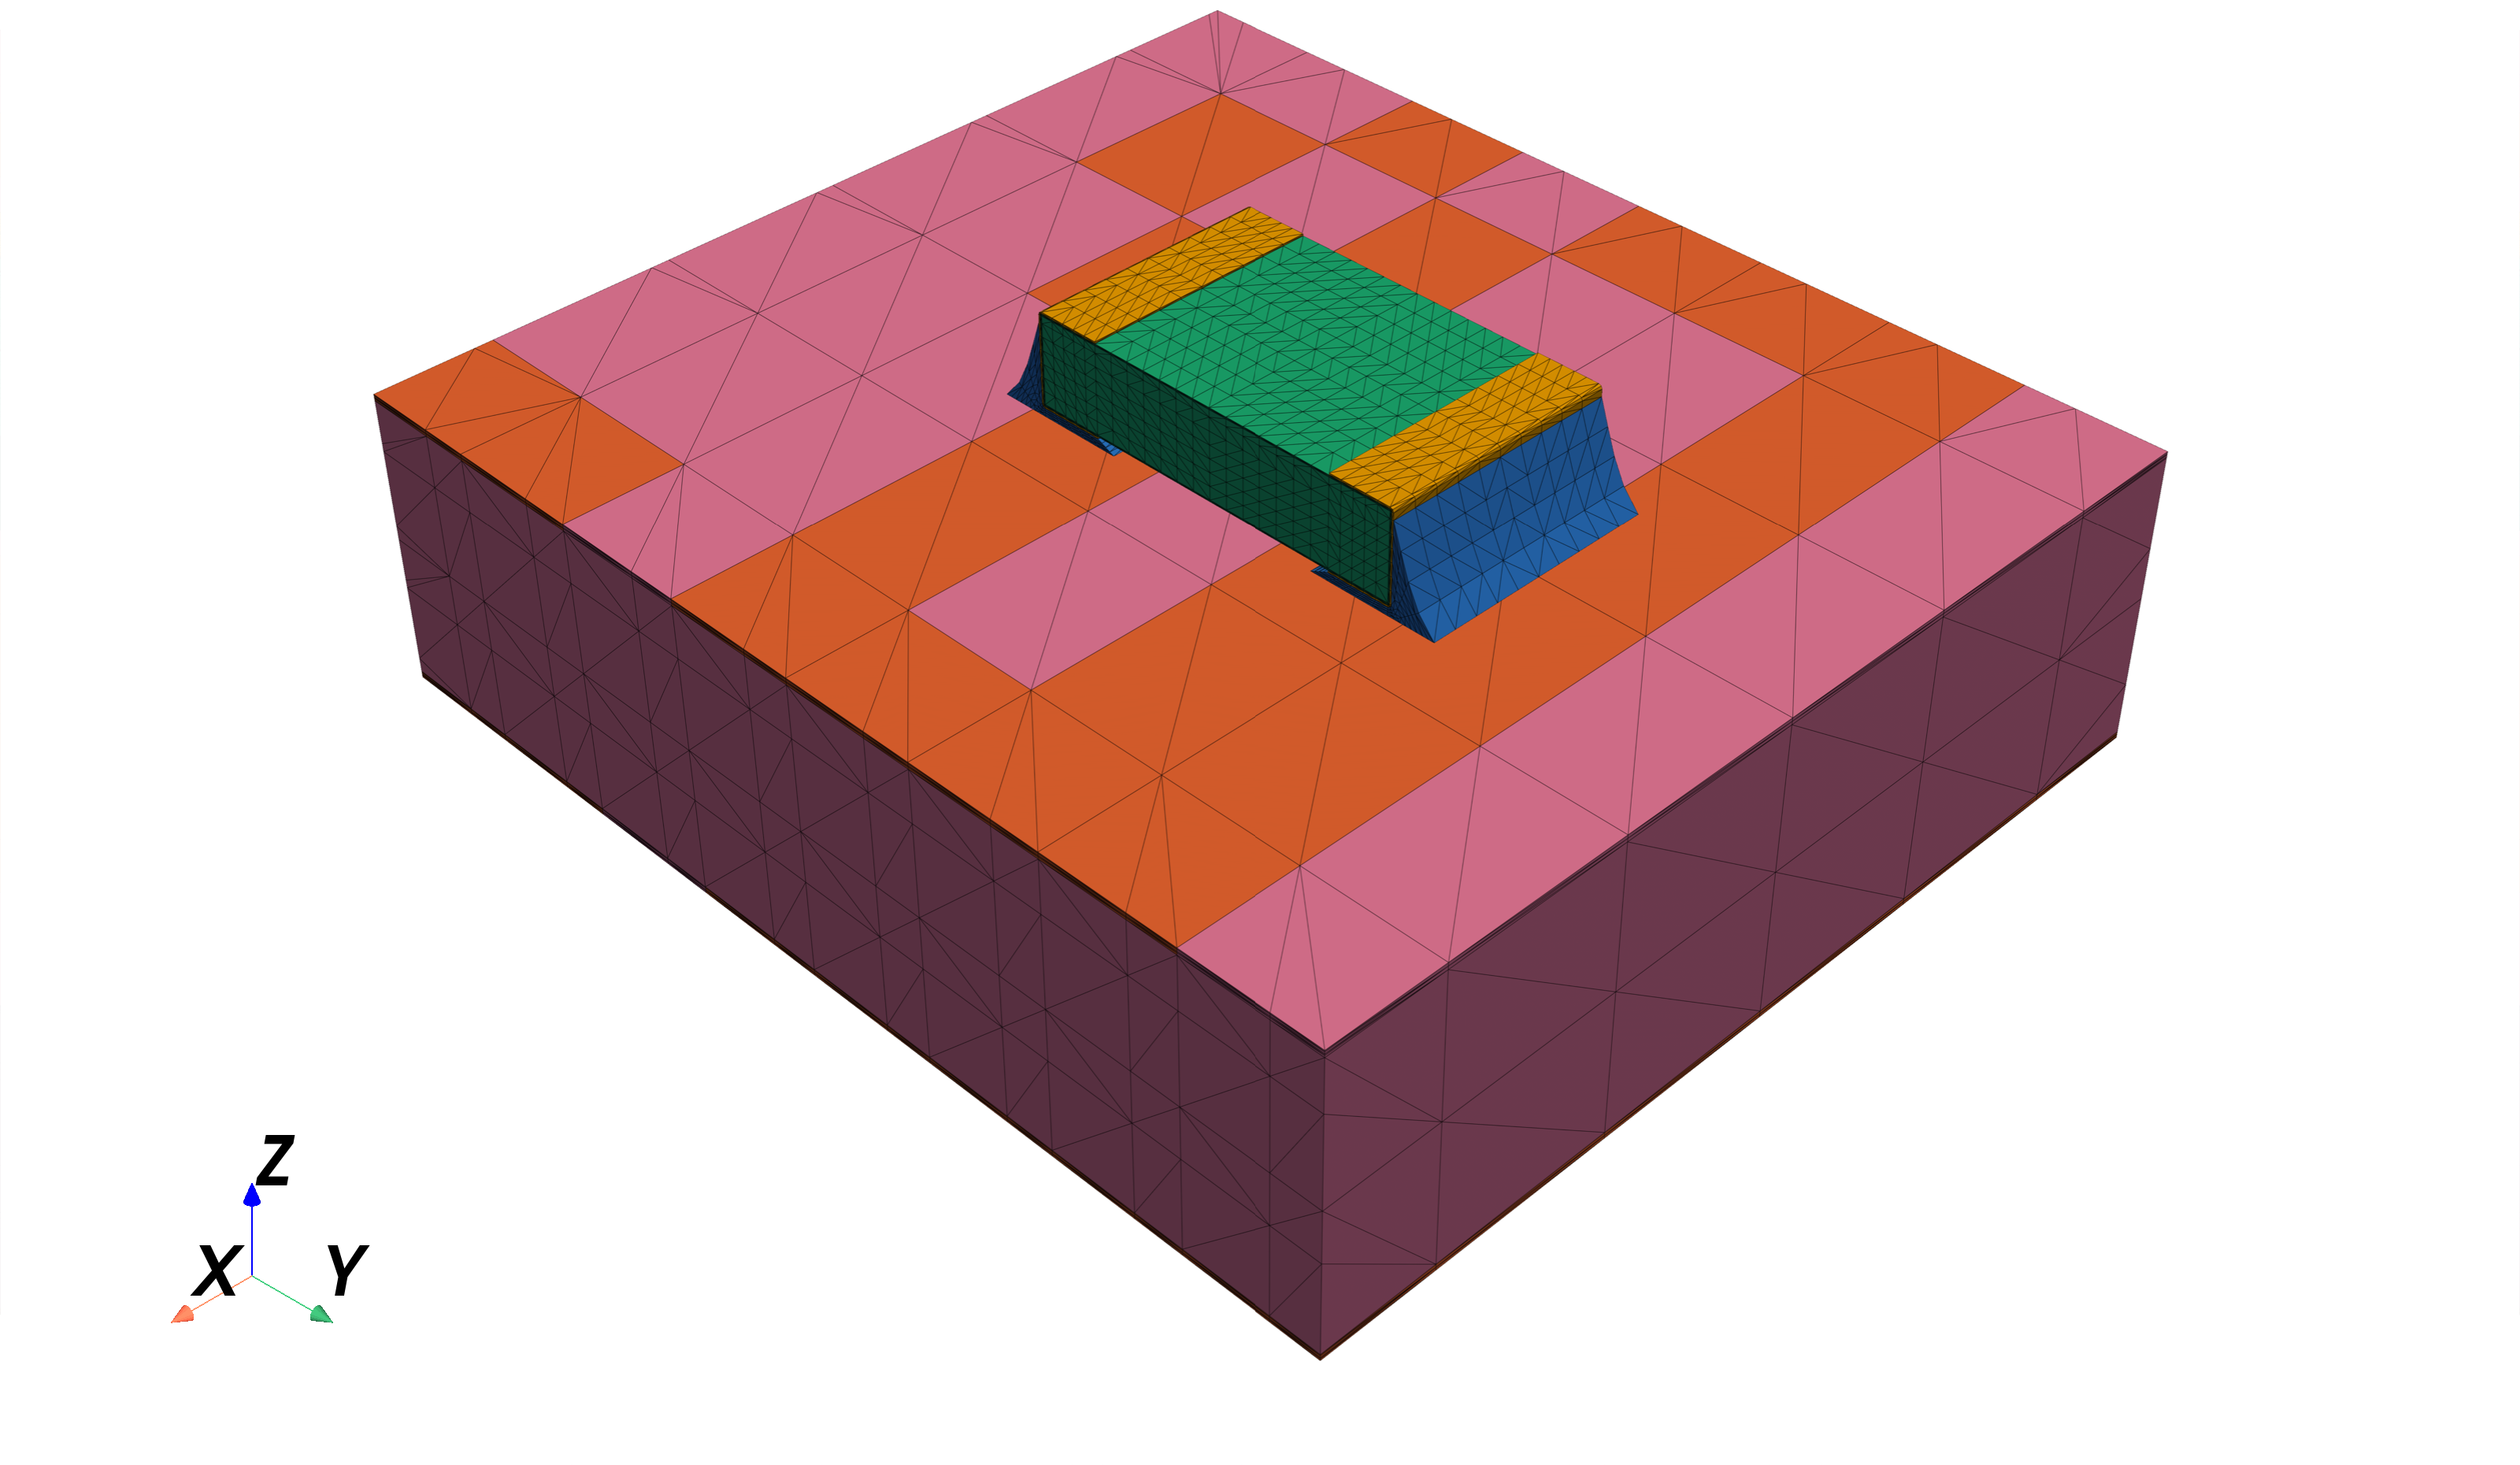
\includegraphics[width=0.72\linewidth]{figures/component_materials.png}
  \caption{Assembly around R1, coloured by material (\code{plot\_component\_materials.py}): ceramic body
  (green, MAT 2), nickel terminations (yellow, MAT 6), SAC305 solder fillets (blue, MAT 9), board copper
  (orange, MAT 9001) and FR4 (pink, MAT 9002) at \numproduct{20 x 20} board resolution.}
  \label{fig:component}
\end{figure}

\newpage
% ---------------------------------------------------------------------------
\section{Thermal load}
\mod{thermal\_profile.py} reads a list of (time, temperature) points and applies them as a uniform
temperature field from a MAPDL time table, so every substep sees the exact profile temperature; each segment
is solved as its own load step. TREF is \SI{180}{\celsius}, the upper end of the solder's material data, and
the example profile starts there, so the solve begins from an undeformed, stress-free state.
The profile is plotted before the solve (\code{results/thermal\_profile.png}, or standalone via
\code{python thermal\_profile.py <profile.yaml>}) and saved next to the results; its cold-hold starts are the
cycle boundaries used below.

\begin{figure}[H]
  \centering
  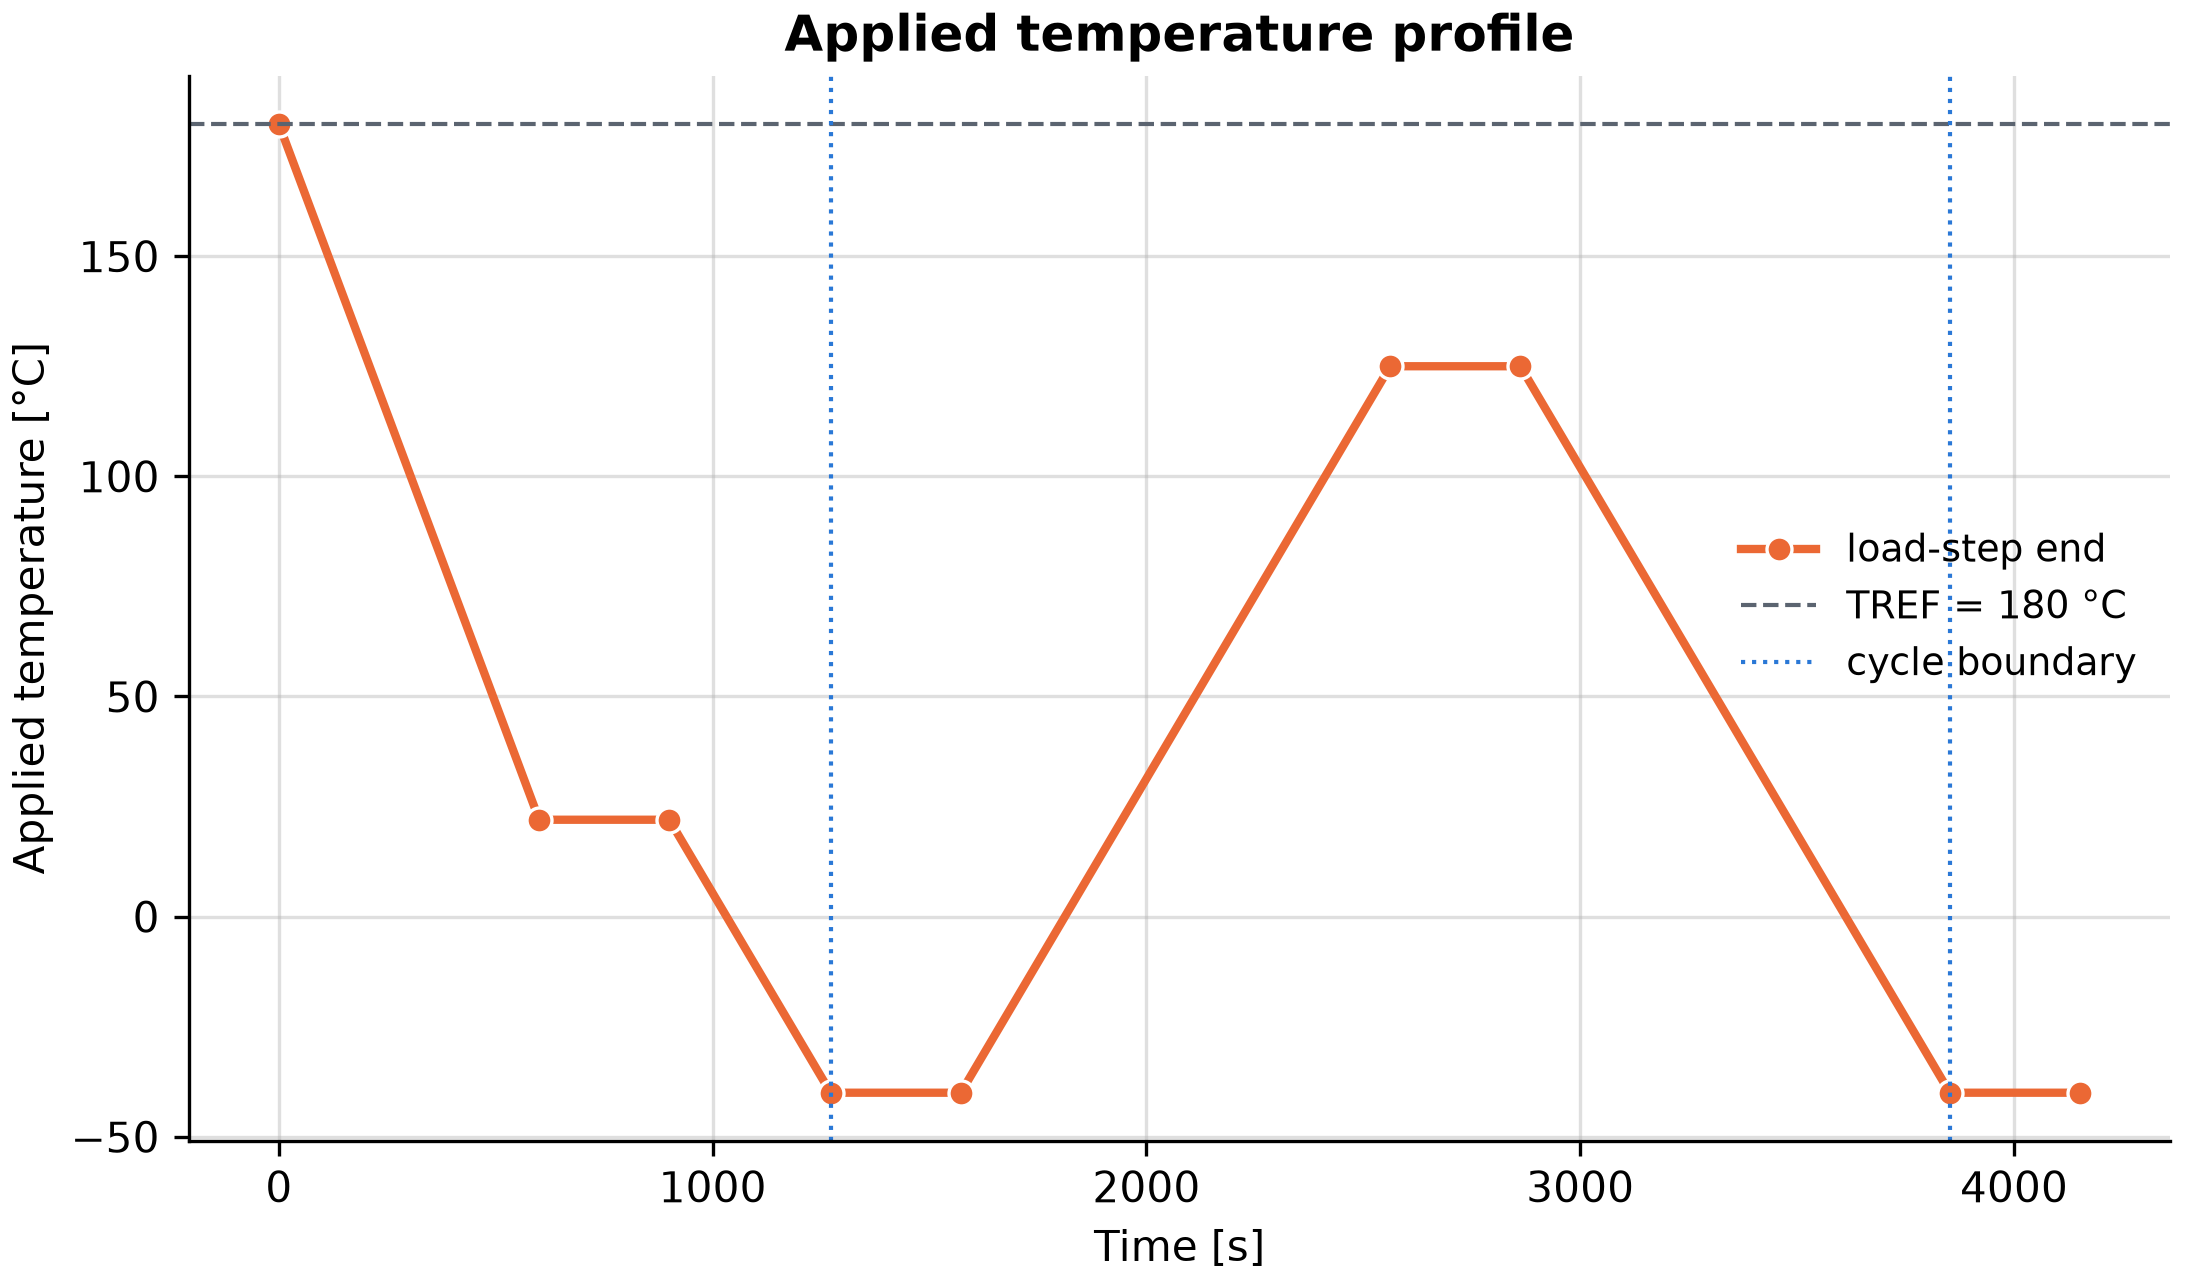
\includegraphics[width=0.66\linewidth]{figures/thermal_profile.png}
  \caption{Applied load of the example profile: cool-down from \SI{180}{\celsius} in \SI{600}{\second},
  \SI{300}{\second} hold at room temperature, then one thermal cycle with \SI{300}{\second} holds. Markers are
  load-step ends; dotted lines are the cycle boundaries.}
  \label{fig:temp}
\end{figure}

\section{Creep post-processing}
All post-processing reads the \code{.rst} directly (ansys-mapdl-reader); no MAPDL session or licence is
needed. \mod{zone\_creep\_strain.py} selects the critical solder sub-volume (here \SI{25}{\percent} of the
solder volume with the highest accumulated creep strain, NL,CREQ) and volume-averages its creep strain over
time, following R.~Schwerz's (Fraunhofer IKTS) APDL macro and Darveaux's method.

\begin{figure}[H]
  \centering
  \begin{subfigure}[c]{0.49\linewidth}
    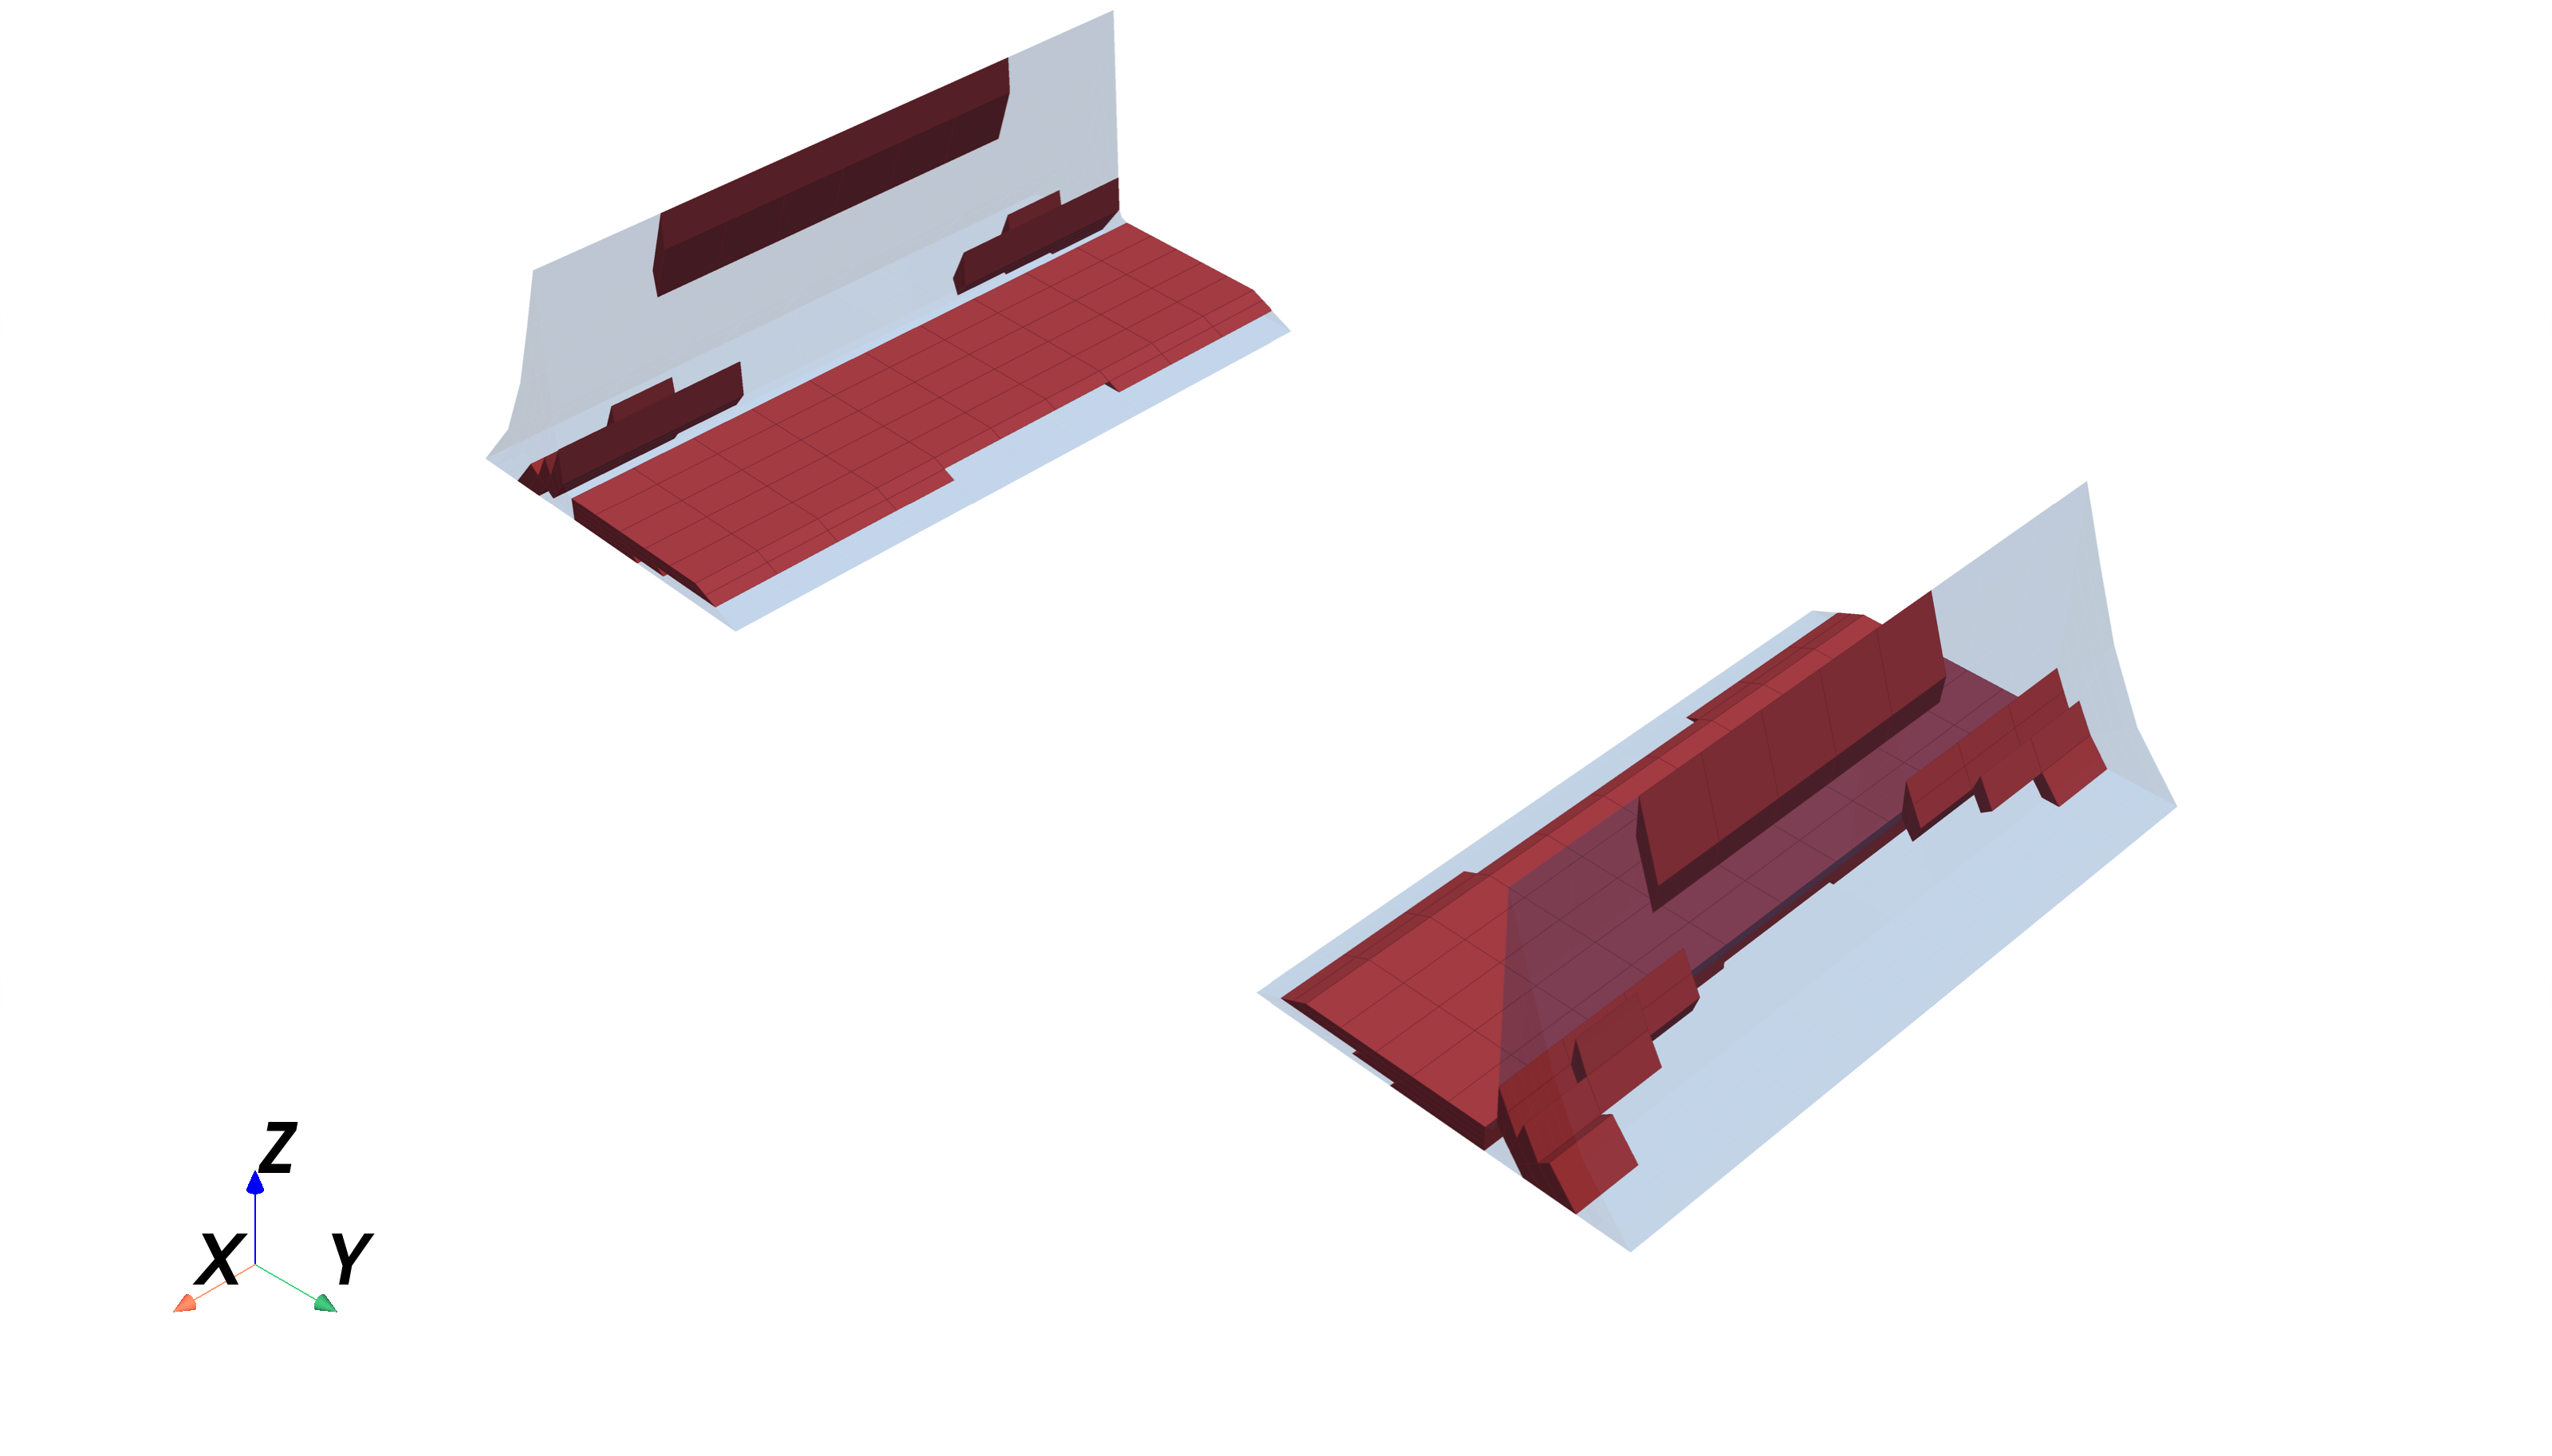
\includegraphics[width=\linewidth]{figures/zone_elements.png}
  \end{subfigure}\hfill
  \begin{subfigure}[c]{0.49\linewidth}
    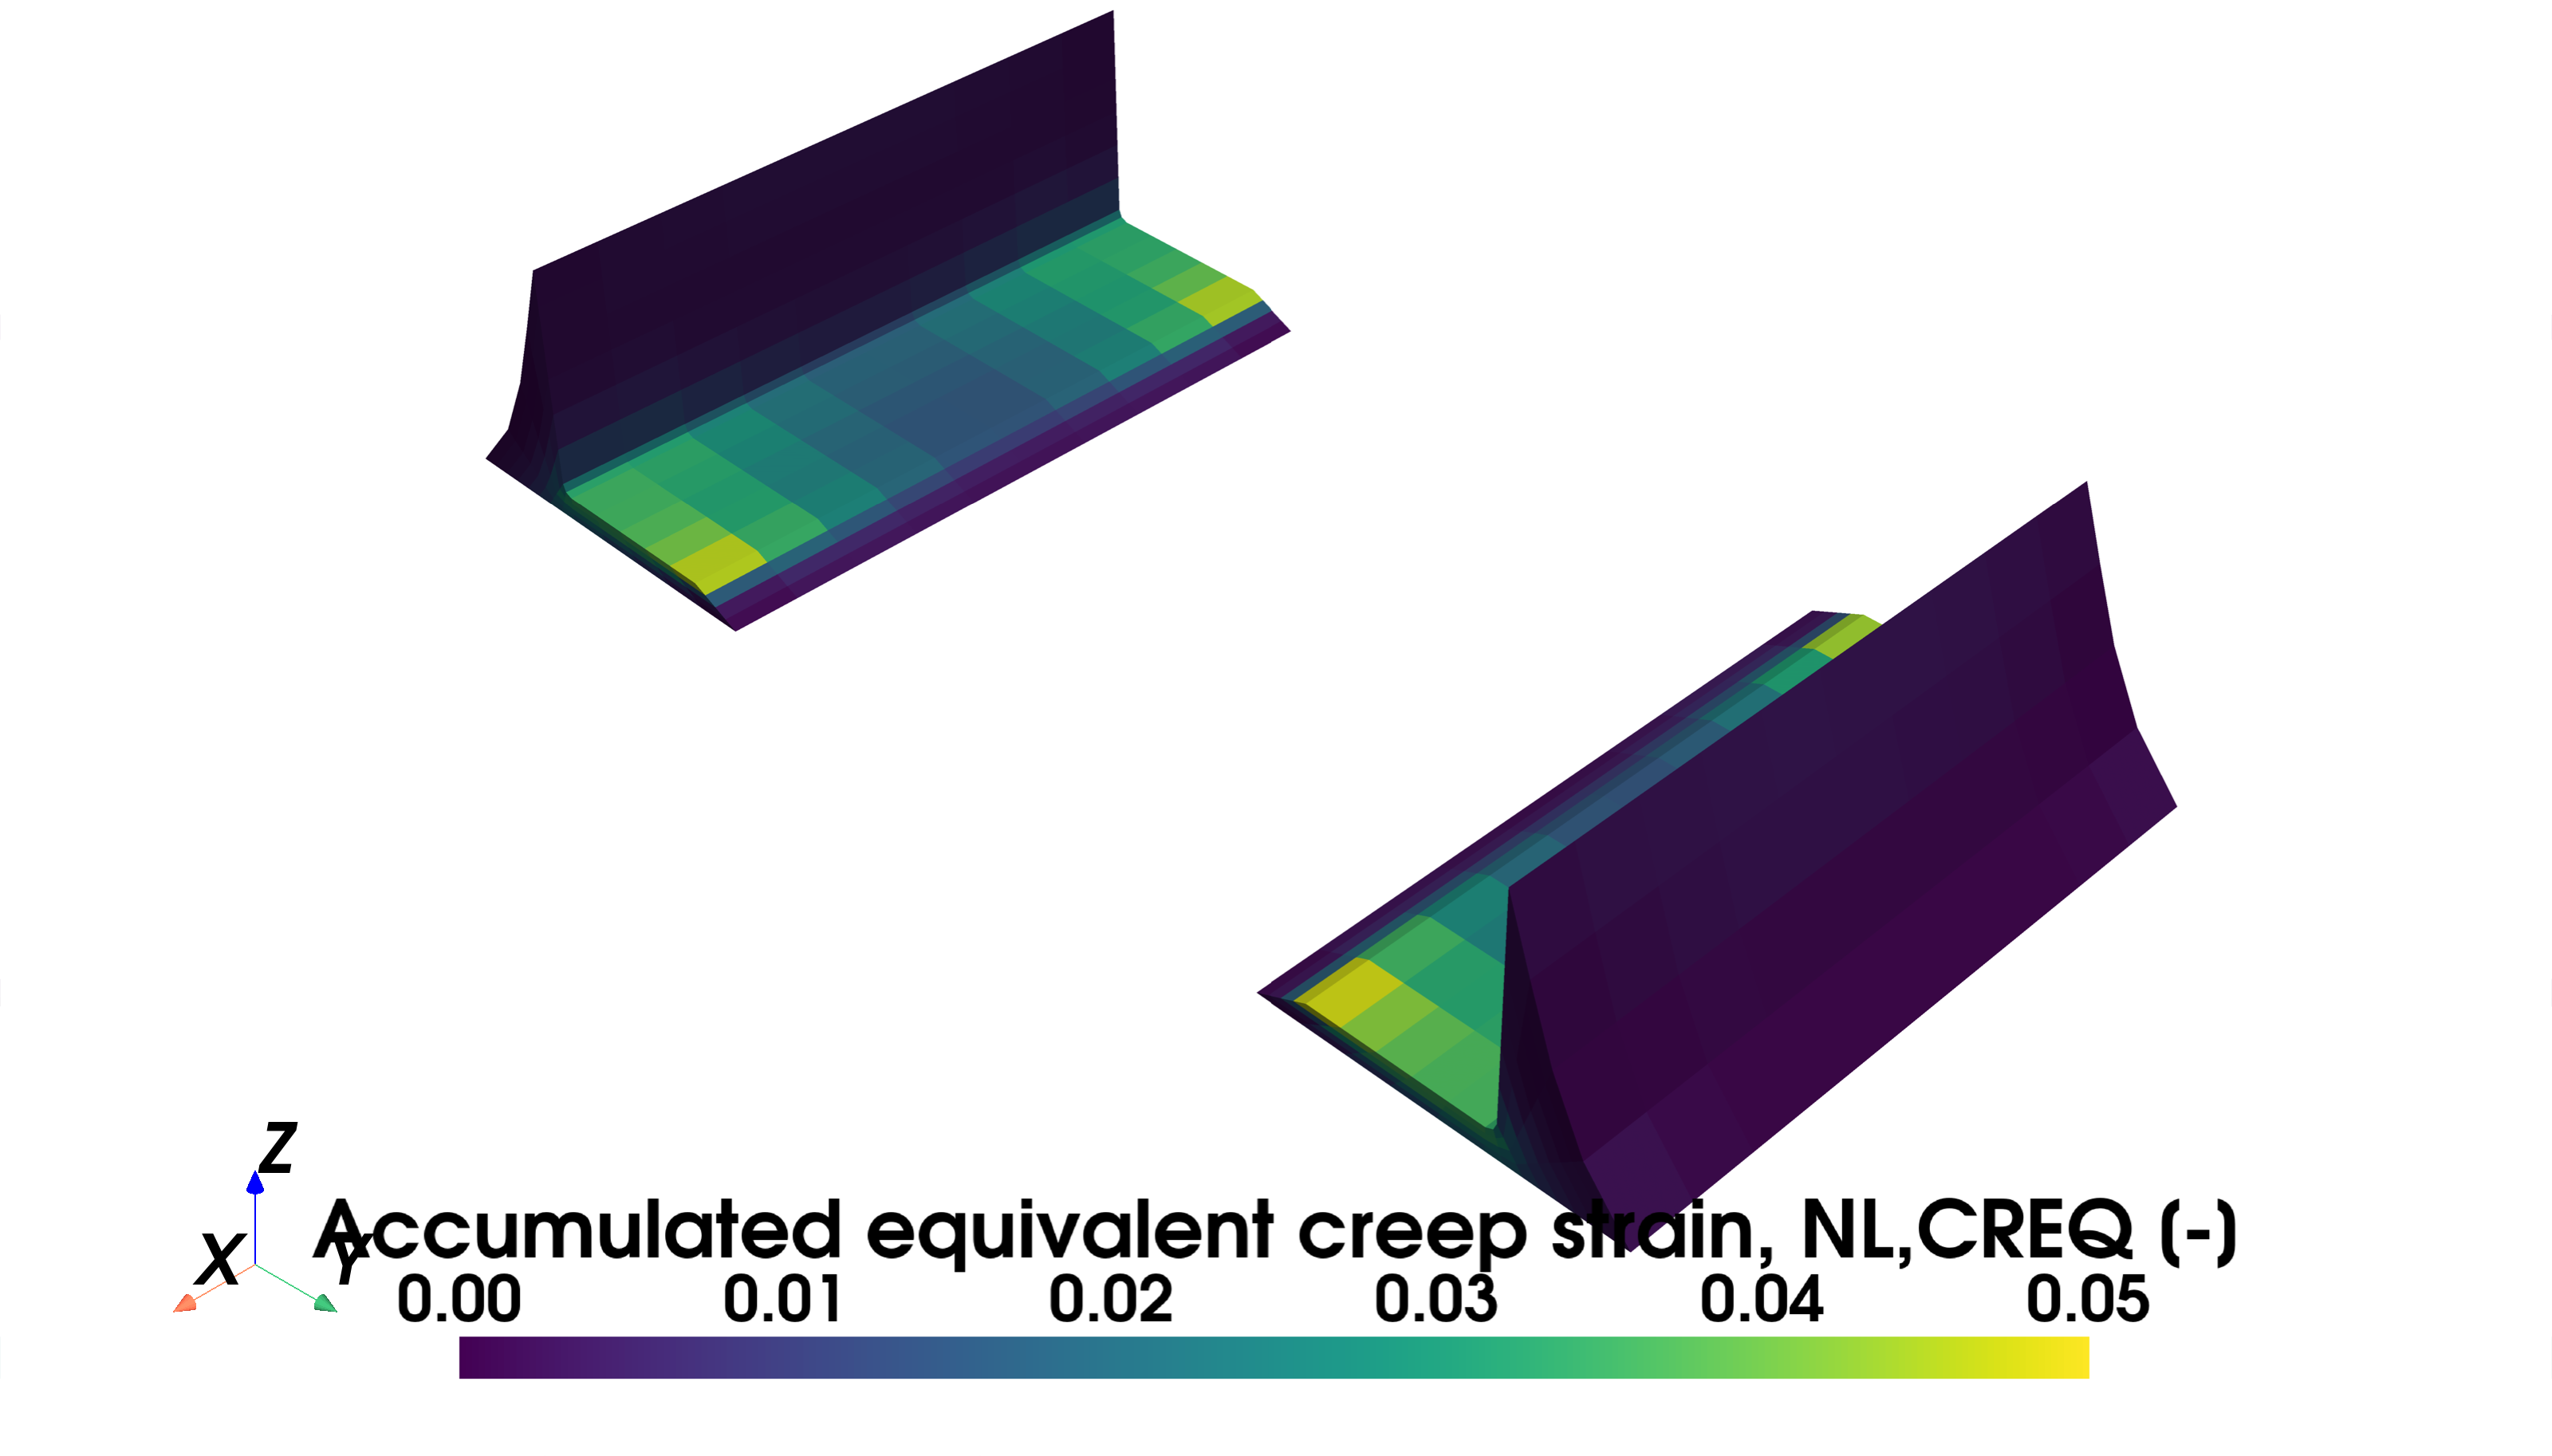
\includegraphics[width=\linewidth]{figures/creep_strain_field.png}
  \end{subfigure}
  \caption{Critical zone: 346 of 1040 solder elements (left) and accumulated creep strain at the end of
  the run (right), both from \code{zone\_creep\_strain.py}.}
  \label{fig:zone}
\end{figure}

\mod{plot\_cycle\_creep\_increment.py} cuts the zone-averaged history at the thermal-cycle boundaries and
reports the creep-strain increment per cycle, the $\Delta\varepsilon$ that enters a Coffin--Manson-type
fatigue law. Plotting every cycle shows whether the response has stabilized (shakedown) before a value is
picked.

\begin{figure}[H]
  \centering
  \begin{subfigure}[c]{0.55\linewidth}
    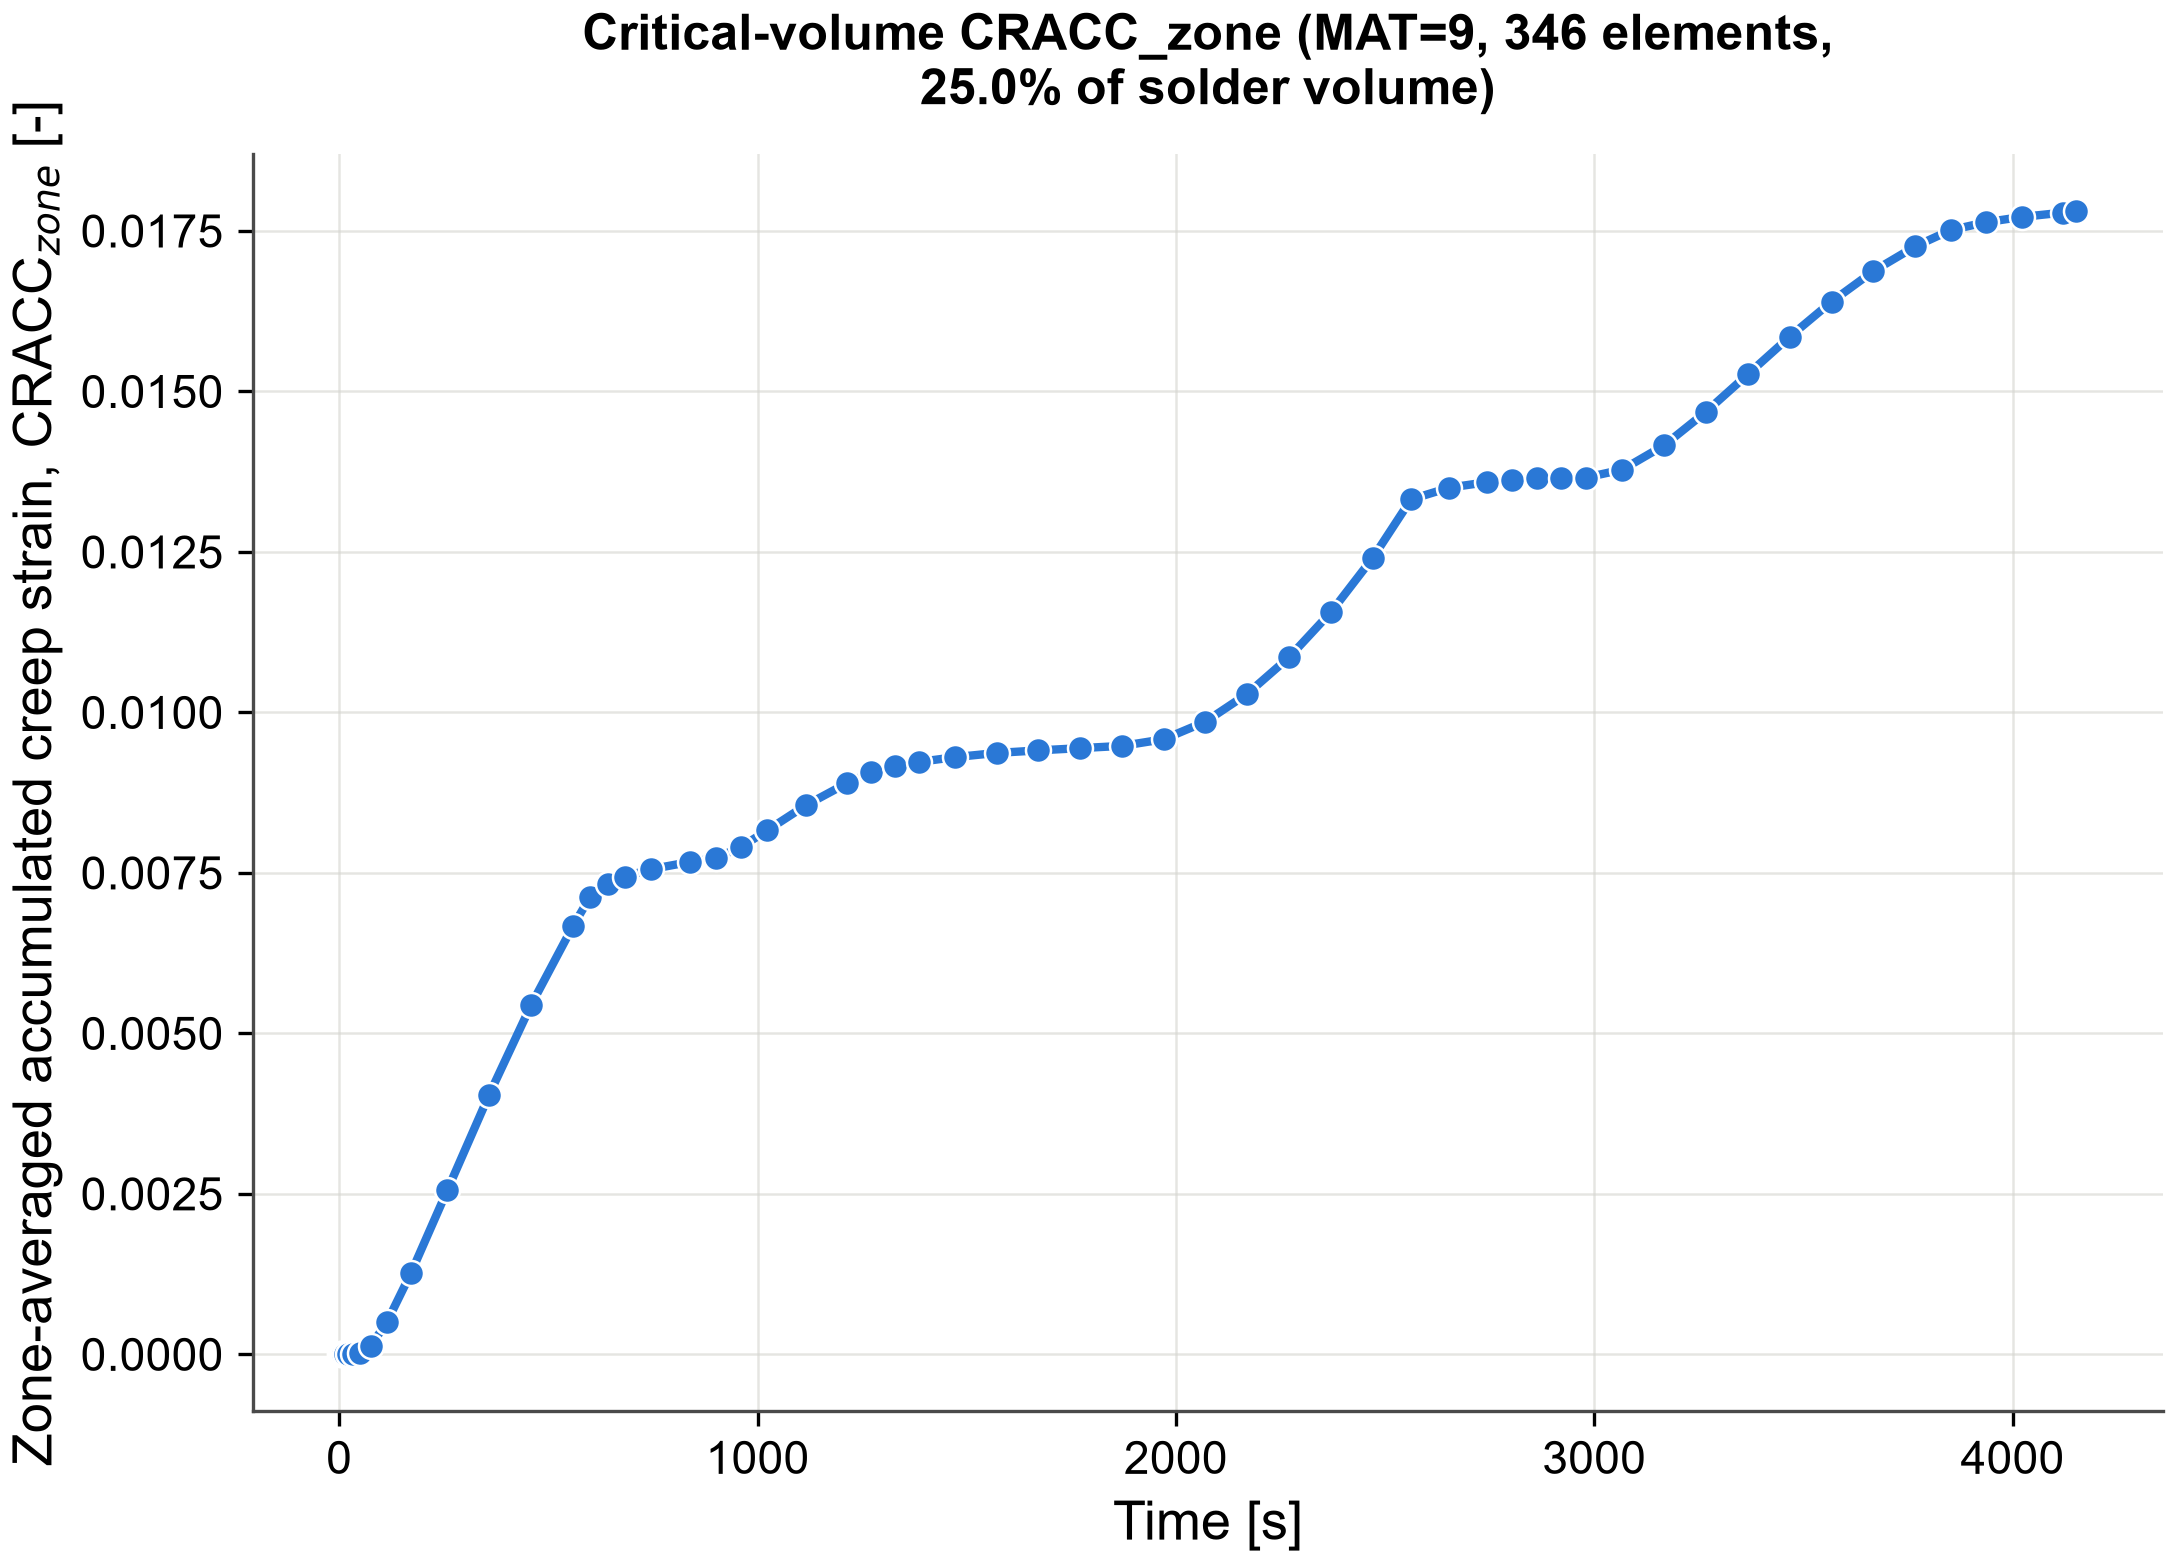
\includegraphics[width=\linewidth]{figures/zone_creep_strain.png}
  \end{subfigure}\hfill
  \begin{subfigure}[c]{0.43\linewidth}
    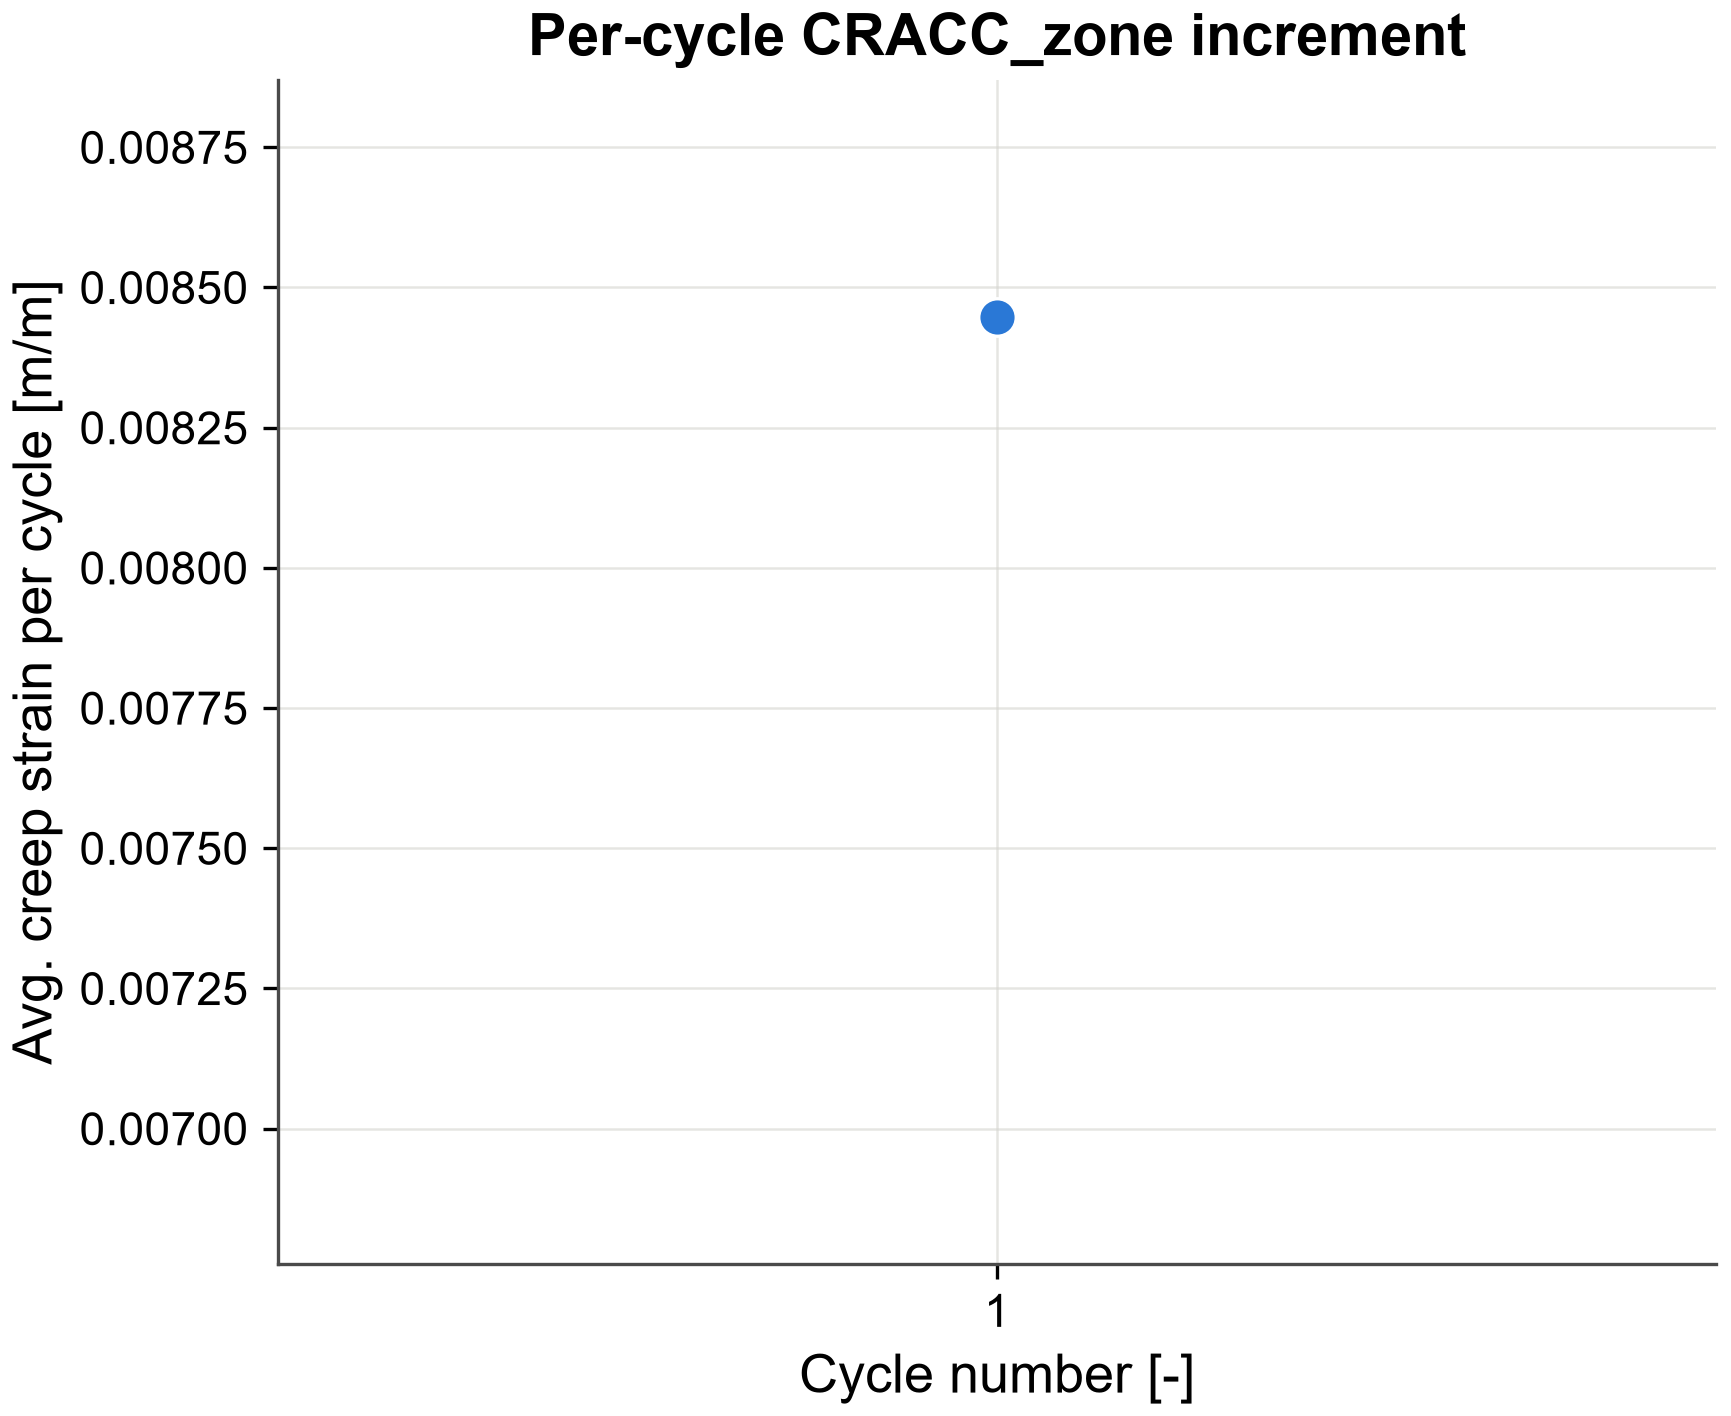
\includegraphics[width=\linewidth]{figures/cycle_creep_increment.png}
  \end{subfigure}
  \caption{Zone-averaged accumulated creep strain vs.\ time (left) and its per-cycle increment (right):
  $\Delta\varepsilon = \num{8.4e-3}$ for the single cycle of the example run.}
  \label{fig:cycle}
\end{figure}

The example run demonstrates the workflow. With one cycle, short holds and a coarse \numproduct{20 x 20}
board mesh that loses most traces under the joint (Fig.~\ref{fig:mapping}), its $\Delta\varepsilon$ is not a
fatigue value: use the full profile, several cycles and the default mesh for that.

\section{Board-model comparison}
\mod{plot\_comparison\_creep.py} overlays the zone-averaged creep history and per-cycle $\Delta\varepsilon$ of
several \mod{simulate\_pyansys\_assembly.py} runs on the same board, read back from their saved
\code{results/} JSON (no \code{.rst} access needed). \code{--board-model homogenized} gives each board
element the orthotropic Voigt--Reuss material of its quadtree leaf, smeared through the full thickness;
\code{homogenized\_zlayers} instead resolves the two copper layers separately -- each gets its own per-leaf
material from \code{phi\_bot}/\code{phi\_top} alone, and the FR4 core in between stays plain FR4. Both need
\code{mesh/quadtree.json} from \mod{quadtree.py}.

\begin{figure}[H]
  \centering
  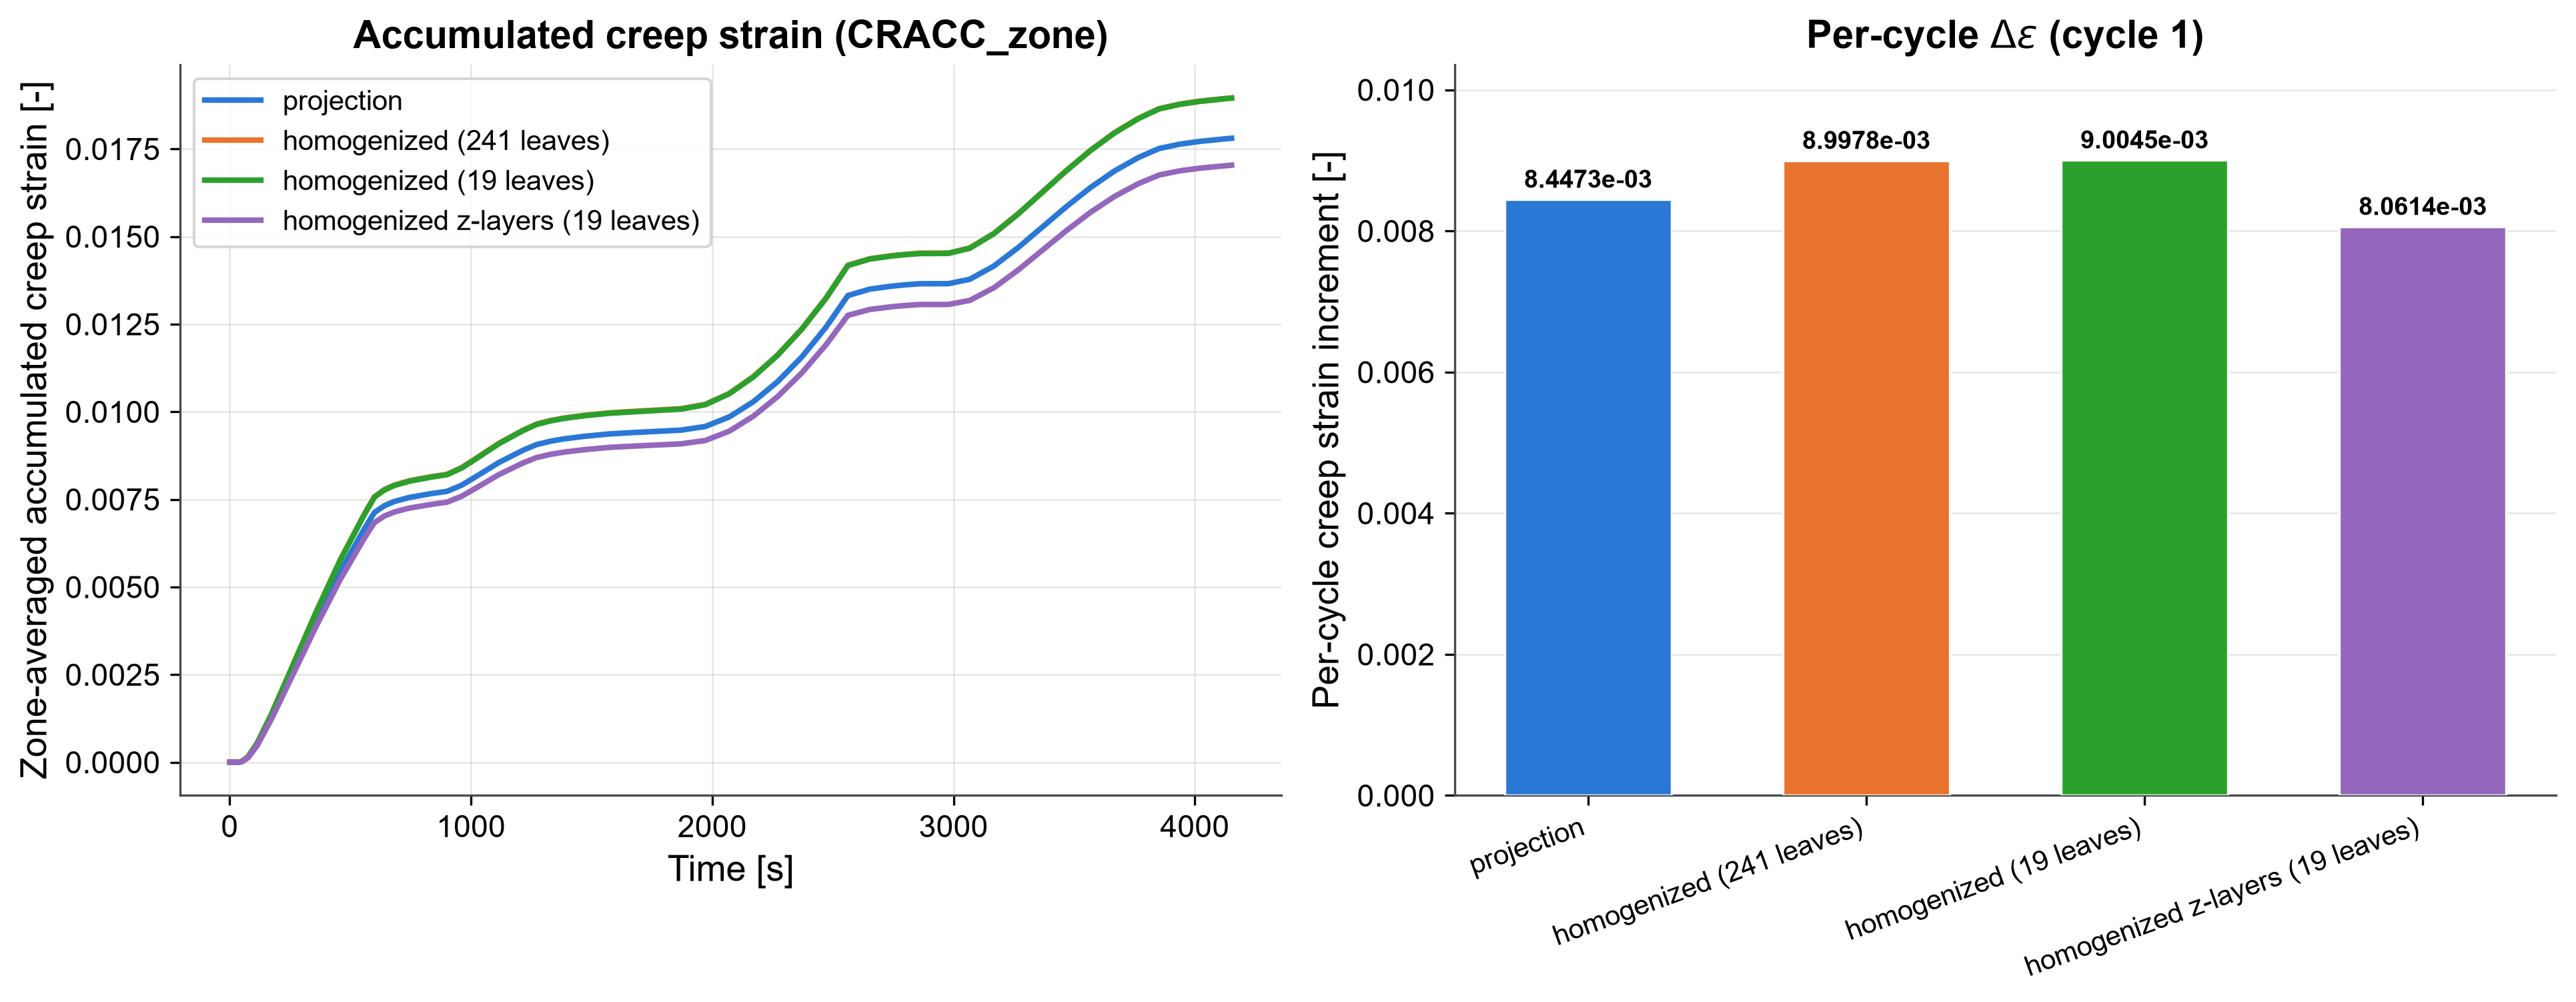
\includegraphics[width=\linewidth]{figures/comparison_creep.png}
  \caption{Zone-averaged accumulated creep strain vs.\ time (left) and the per-cycle increment (right) across
  four board models of the same \code{rv3032\_example} board: the directly projected copper/FR4 raster,
  full-resolution homogenization (241 leaves), the coarser 19-leaf quadtree, and the same 19-leaf quadtree
  with the two copper layers homogenized separately (\code{homogenized\_zlayers}). The coarse quadtree
  tracks the full-resolution homogenization closely ($\Delta\varepsilon=\num{9.00e-3}$ vs.\
  \num{9.00e-3}, both $\sim$\SI{6.5}{\percent} above the projection's \num{8.45e-3}), while resolving
  the copper layers separately pulls $\Delta\varepsilon$ below the projection instead (\num{8.06e-3},
  $-4.6\,\%$) -- smearing both layers into one orthotropic material over- or under-stiffens the joint
  differently than keeping them apart.}
  \label{fig:comparison}
\end{figure}

\end{document}
